\documentclass[border=4pt]{standalone}
\usepackage{fontspec}
\usepackage{amsmath}
\usepackage{unicode-math}
\setmainfont{Latin Modern Roman}
\setmathfont{Latin Modern Math}
\usepackage{pgfplots}
\usepackage{pgfplotstable}
\pgfplotsset{compat=1.18}
\usepackage{tkz-euclide}
\usetikzlibrary{arrows.meta,calc,angles,quotes,patterns,3d,backgrounds}
\definecolor{ink}{HTML}{123428}
\definecolor{asy}{HTML}{475569}
\definecolor{mint}{HTML}{86e0bd}
\tikzset{asym/.style={asy, line width=0.9pt, dash pattern=on 5pt off 3.5pt},
         guide/.style={gray!70, line width=0.6pt, densely dotted},
         dot/.style={circle, inner sep=0pt, minimum size=5pt, draw=white, line width=0.5pt},
         odot/.style={circle, inner sep=0pt, minimum size=5.5pt, fill=white, line width=1pt},
         lab/.style={font=\footnotesize, inner sep=1.5pt, text=ink}}
\begin{document}
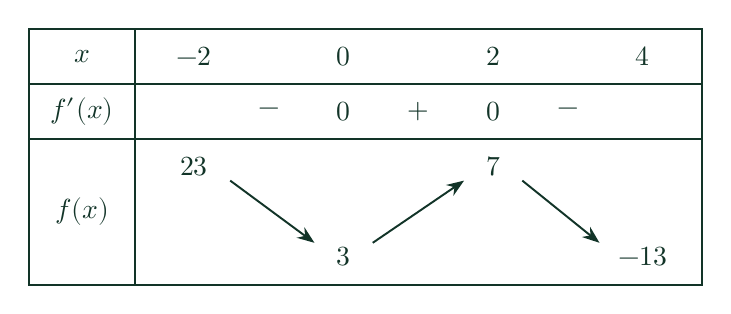
\begin{tikzpicture}
\draw[ink, line width=0.7pt] (0,0) rectangle (8.55,3.25);
\draw[ink, line width=0.6pt] (0,2.55) -- (8.55,2.55);
\draw[ink, line width=0.6pt] (0,1.85) -- (8.55,1.85);
\draw[ink, line width=0.6pt] (1.35,0) -- (1.35,3.25);
\node[text=ink] at (0.68,2.90) {$x$};
\node[text=ink] at (0.68,2.20) {$f'(x)$};
\node[text=ink] at (0.68,0.93) {$f(x)$};
\node[text=ink] at (2.10,2.90) {$-2$};
\node[text=ink] at (2.10,1.50) {$23$};
\node[text=ink] at (4.00,2.90) {$0$};
\node[text=ink] at (4.00,2.20) {$0$};
\node[text=ink] at (4.00,0.35) {$3$};
\node[text=ink] at (5.90,2.90) {$2$};
\node[text=ink] at (5.90,2.20) {$0$};
\node[text=ink] at (5.90,1.50) {$7$};
\node[text=ink] at (7.80,2.90) {$4$};
\node[text=ink] at (7.80,0.35) {$-13$};
\node[text=ink] at (3.05,2.20) {$-$};
\draw[ink, line width=0.7pt, -{Stealth[length=2.2mm]}] (2.56,1.32) -- (3.63,0.53);
\node[text=ink] at (4.95,2.20) {$+$};
\draw[ink, line width=0.7pt, -{Stealth[length=2.2mm]}] (4.37,0.53) -- (5.53,1.32);
\node[text=ink] at (6.85,2.20) {$-$};
\draw[ink, line width=0.7pt, -{Stealth[length=2.2mm]}] (6.27,1.32) -- (7.25,0.53);
\end{tikzpicture}
\end{document}
